\section{Raft Protocol: Consensus Replication}

\label{sec:raft}
\noindent
As we've discussed so far, replication consistency is crucial and a 
difficult task. The next strategy, \textbf{Raft}, deals with such problem.
There are other solutions, however, Raft is considered safe and easier to 
implement correctly than other solutions:
\begin{Def}[State Machines \& Consensus Algorithms]
    
    A \textbf{State Machine} processes sequence of inputs from a \textbf{log} and saves them
    in state.
    \textbf{Replicated state machines} are implemented via \textbf{replicated logs} across multiple servers
    utilizing a \textbf{Consensus Model}, which facilitate data agreement between nodes. 
    
    Hence, commands need be \textbf{deterministic}, and the consensus algorithm 
    \textbf{must be} flexible enough to handle and replicate application specific data.
\end{Def}

\vspace{-1.5em}
\begin{figure}[h]
    \centering
    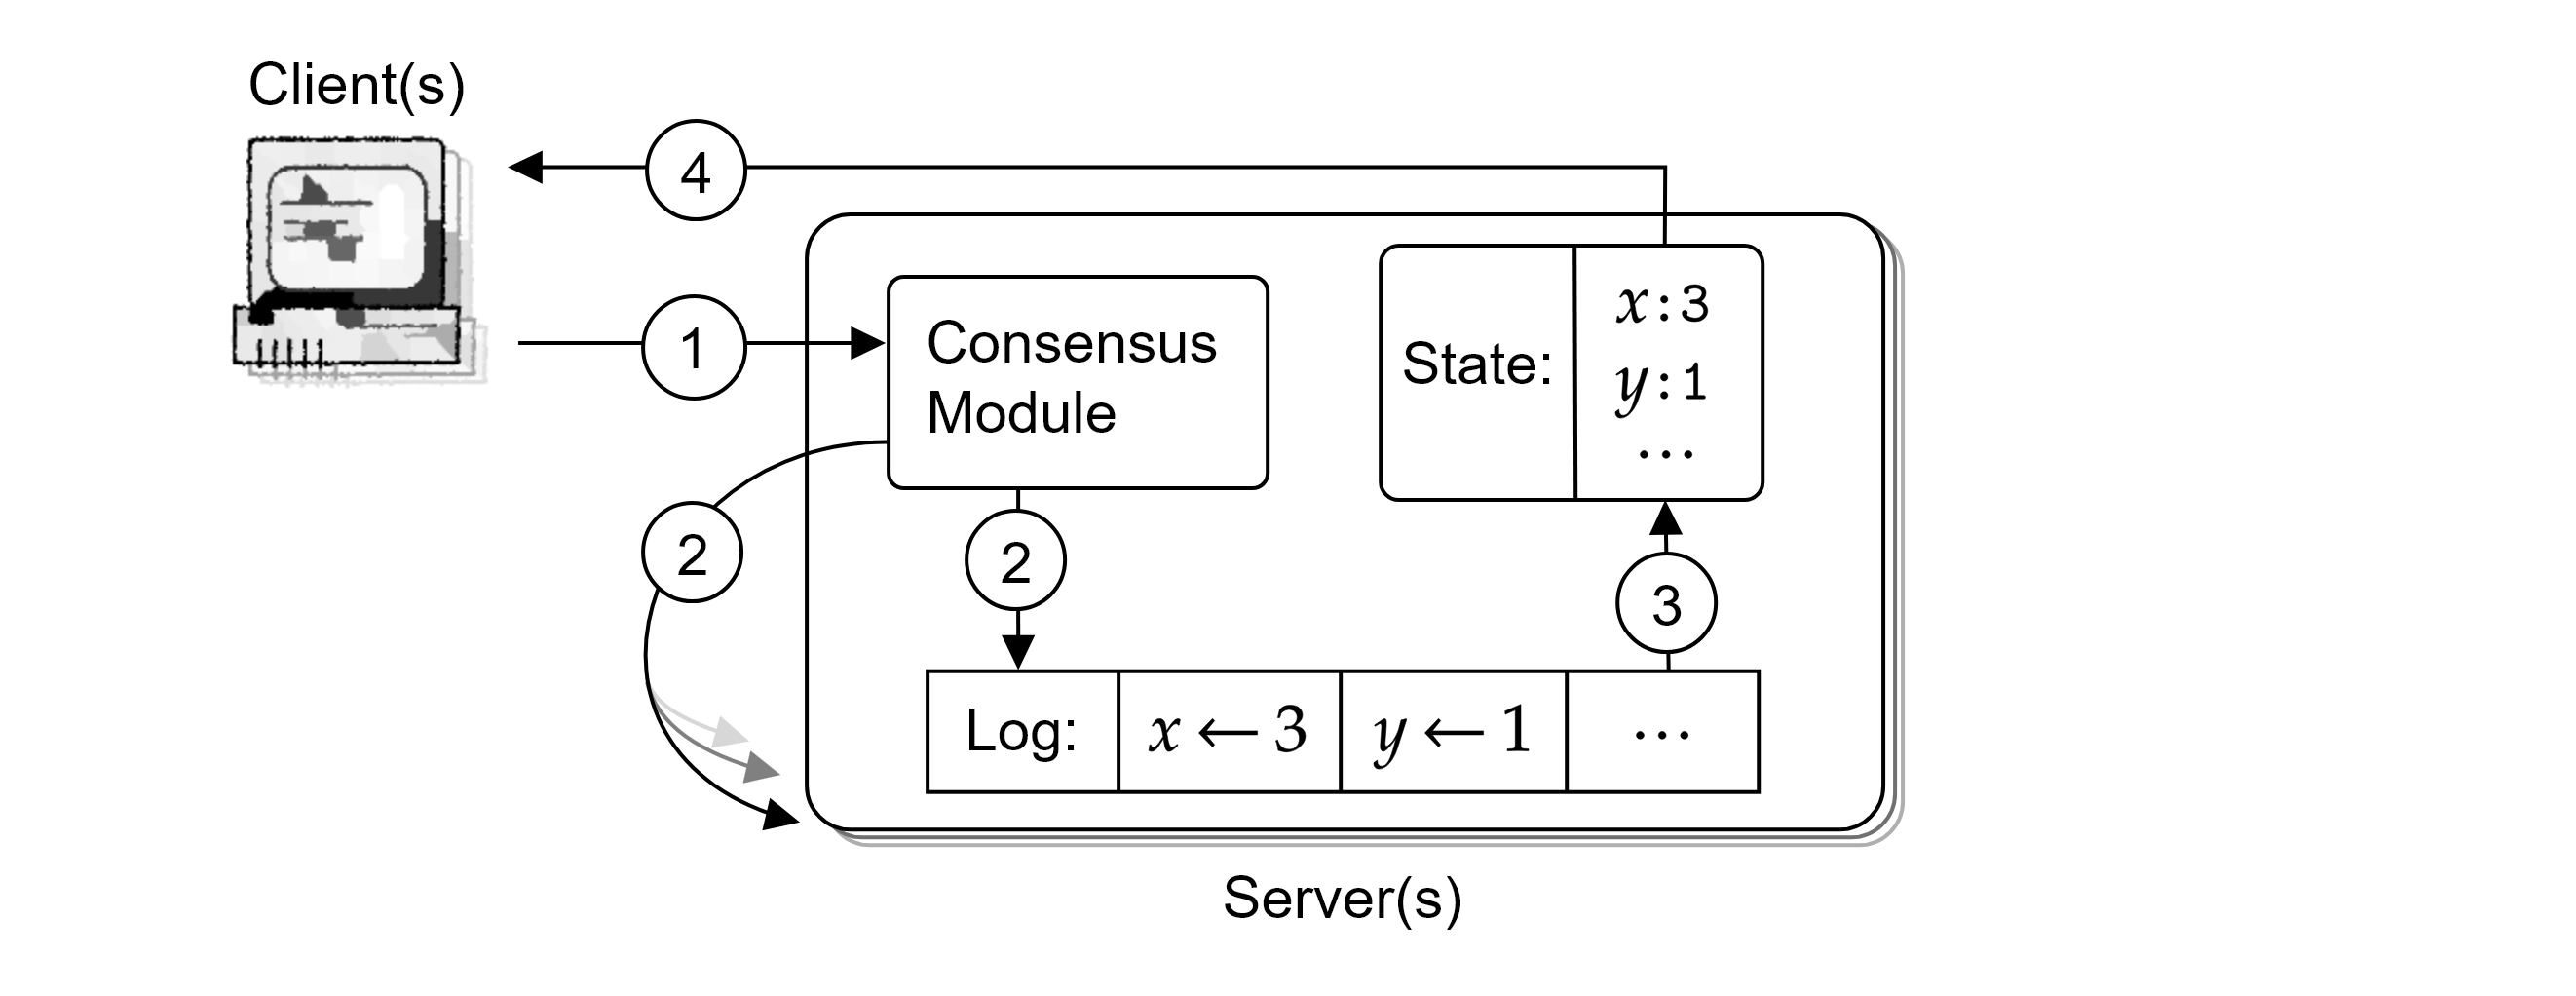
\includegraphics[width=1\textwidth]{Sections/raft/state.png}
    \caption{High-level framework for replicated state machines.}
\end{figure}

\noindent
In the above the \textbf{Consensus Module} communicates with other servers to serve consistent logs. 

\newpage 
\subsection{Procedure Outline: Heartbeats, Elections, \& Log Replication}
\noindent
Now to define the parts which make up a consensus algorithm:
\begin{Def}[Consensus Algorithm Components]

    A \textbf{Consensus Algorithm} involves the following components:
    \begin{itemize}
        \item \textbf{Safety}: Always returns correct results in spite of, network delays, partitions, duplications, and reorderings.
        \item \textbf{Liveness}: A \textbf{Cluster} (group of servers) must tolerate a subset of server failures (e.g., A cluster of 5 servers can tolerate 2 failures). Offline 
        servers may later recover and rejoin the cluster.
        \item \textbf{Time Agnostic}: The algorithm must not rely on synchronized clocks.
        \item \textbf{Majority Rule}: A majority of servers must agree on a value before it is committed. Minority slow servers must not block the system.
    \end{itemize}
\end{Def}

\noindent
At a high level, The Raft Algorithm:
\begin{Def}[Raft Abstract]

    The Raft Algorithm involves three main components:
    \begin{itemize}
        \item \textbf{Leader Election}: A leader $\ell$ is elected to manage the replication process of backups $\beta$.
        \item \textbf{Heartbeats}: Where $\ell$ and $\beta$ exchange consistent pulses of data to ensure liveliness.
        \item \textbf{Assurance}: Commit points (\ref{def:commit}) are established between the client, $\ell$, and $\beta$. 
    \end{itemize}
\end{Def}
\noindent
In Raft, servers are given roles to manage the replication process.
\begin{Def}[Raft Server States]

    A Raft server can be in one of the following states:
    \begin{itemize}
        \item \textbf{Follower}: A server that listens to the leader.
        \item \textbf{Candidate}: A server that is running for leader.
        \item \textbf{Leader}: A server that is managing the replication process.
    \end{itemize}
    \textbf{Followers are passive} and simply listen to the leader.
\end{Def}

\newpage 

\noindent
\begin{Def}[Raft Heartbeats]

    Raft servers exchange \textbf{heartbeats} to ensure liveliness. Each server on boot is randomly assigned a timeout value.
    After the initial timeout, a server sends a signal akin to the out-and-in beats of a heart.
    \textbf{Out-beats} are origin signals, and \textbf{in-beats} are return signals. If a server $\beta$
    receives an out-beat from another server $\ell$ before its in-beat, the $\beta$ timer resets and follows $\ell$'s beat. 
    The leader of the beat's timer is not used.
\end{Def}

\vspace{-.5em}
\begin{figure}[h]
    \centering
    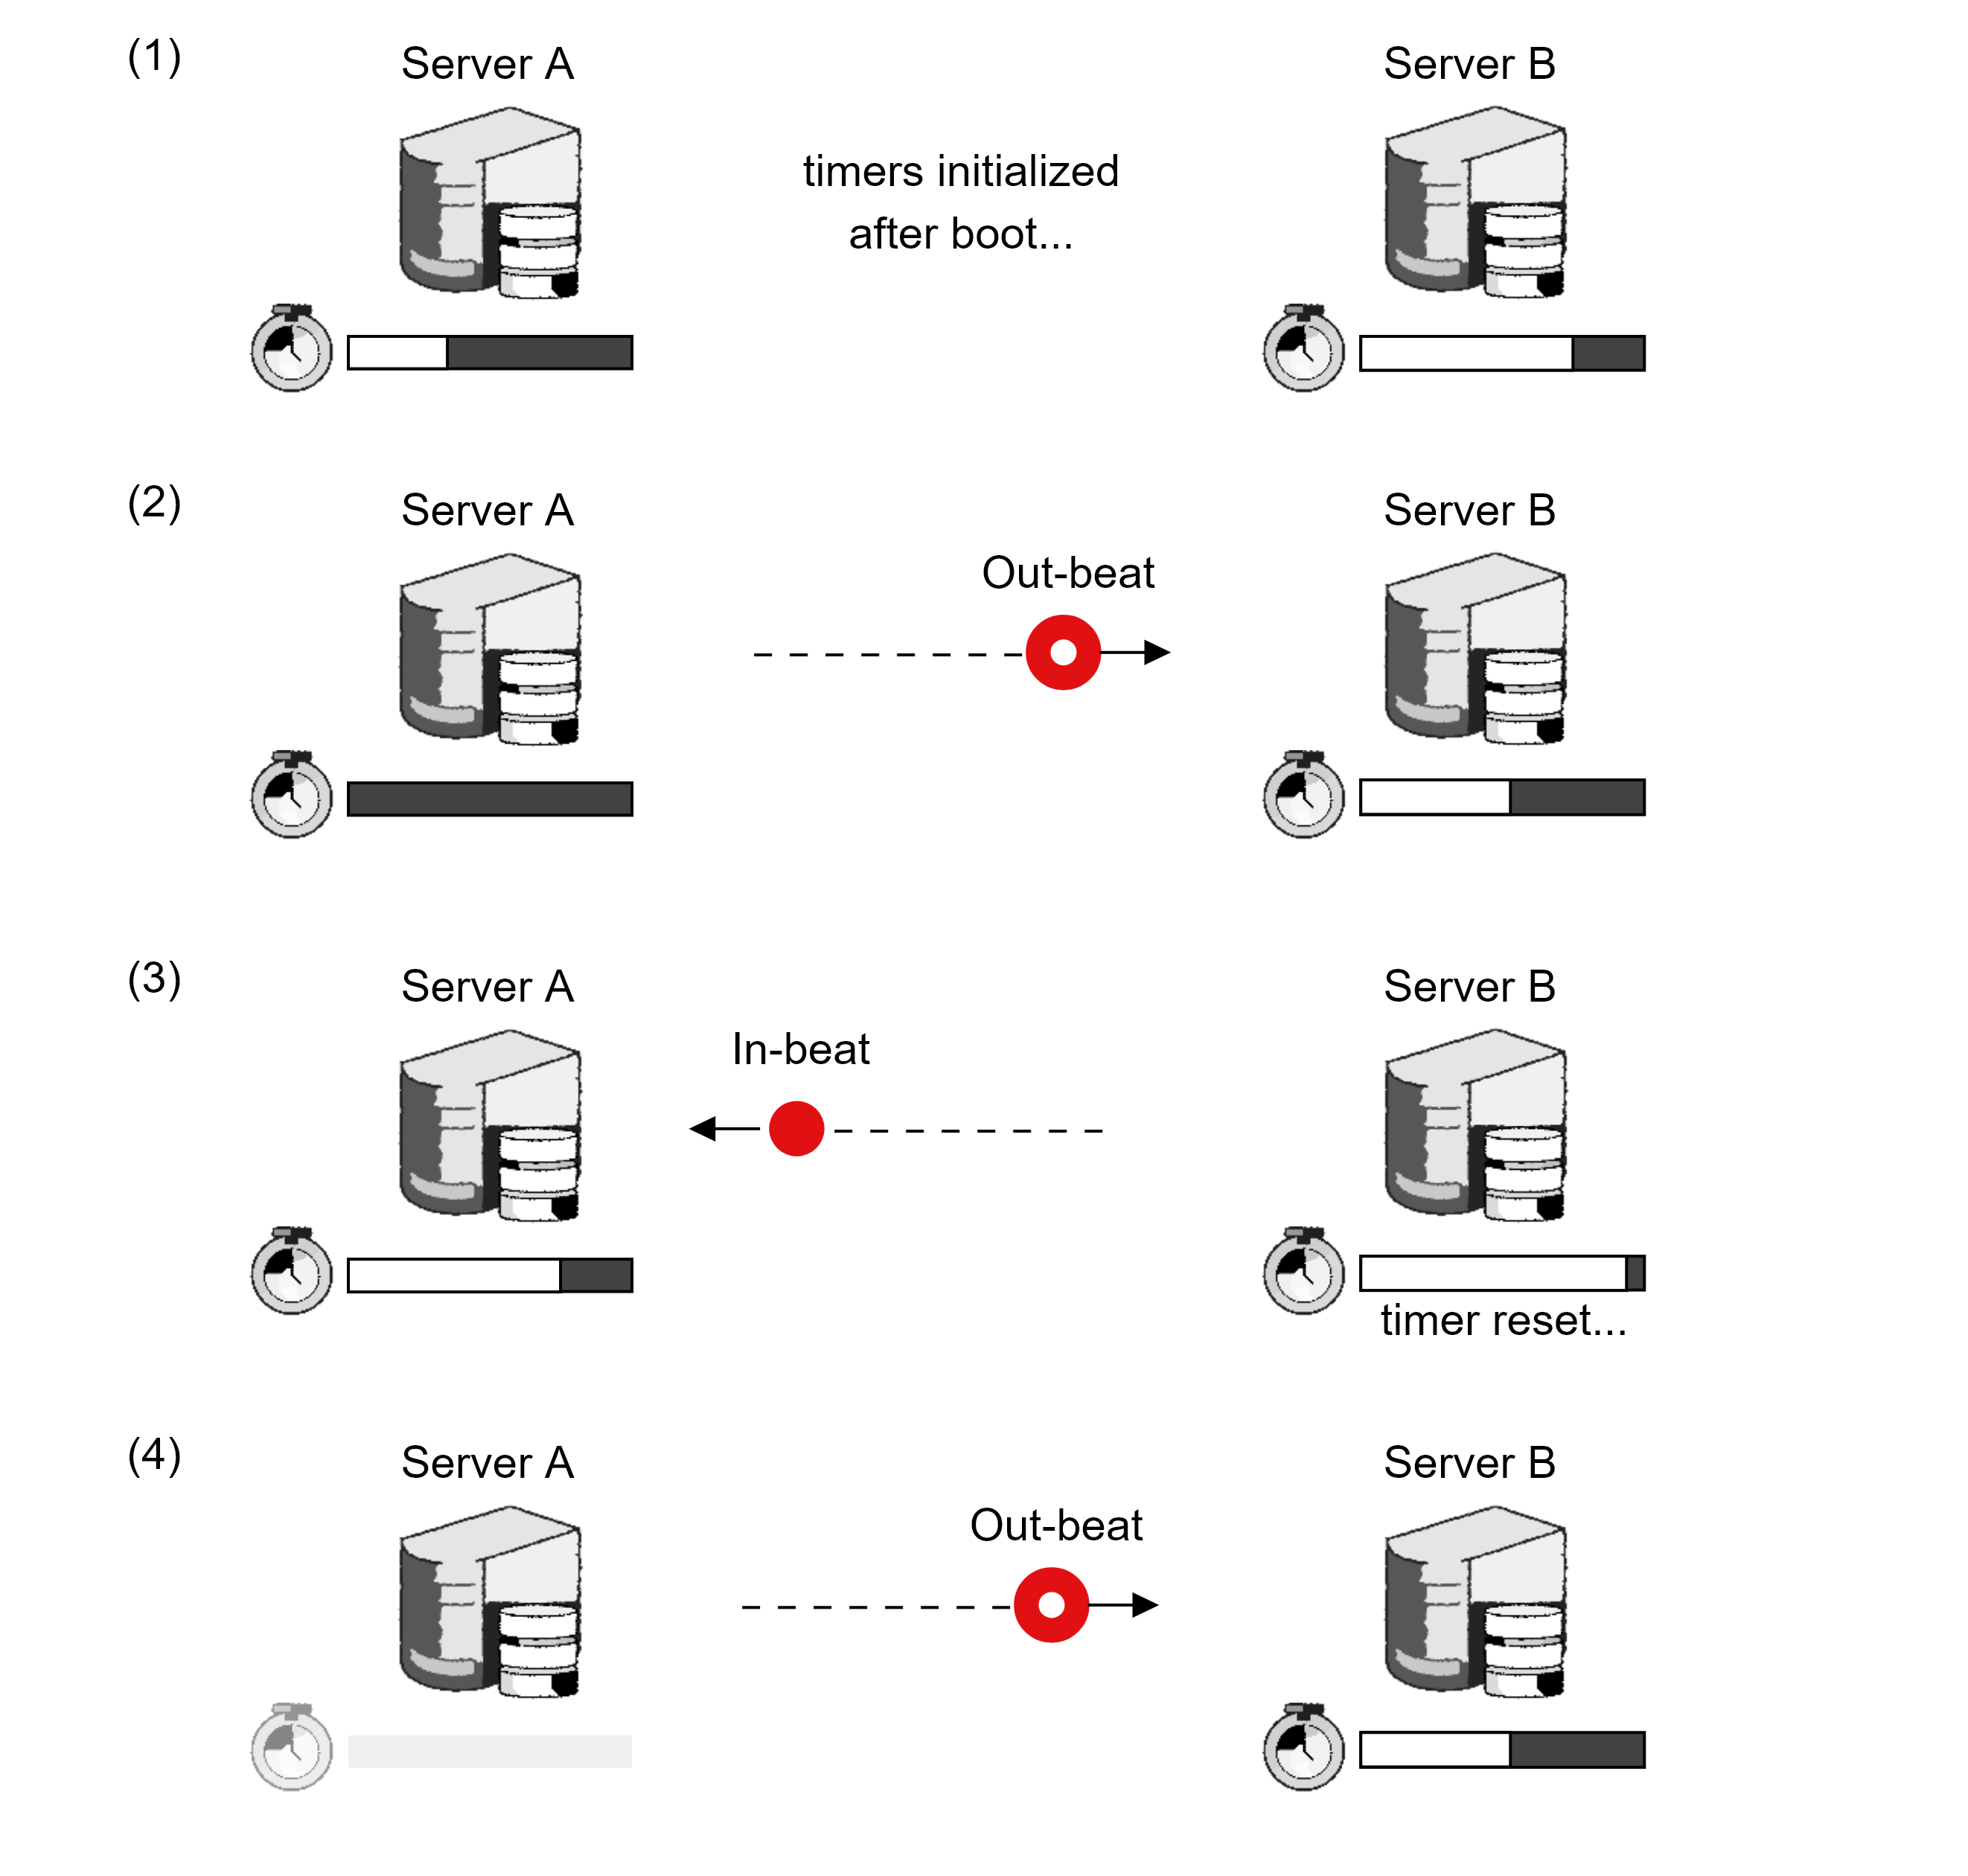
\includegraphics[width=.9\textwidth]{Sections/raft/heart.png}
    \caption{Server $A$ and $B$ exchanging heartbeats after system initialization (1).
    Server $A$'s timer runs out first, sending the first signal to $B$ (2). $B$ has received $A$'s out-beat, and now follows them. $B$ resets
    their timer, and returns the signal to $A$ (3).
    $A$'s timer isn't effect, \textbf{nor is it used} whilst a leader of the beat (4).}
\end{figure}

\newpage

\begin{Def}[Raft Election Terms]

    Let us denote an arbitrary server as $\beta$, then $\beta$ is either of class $\gamma$ (\textbf{Follower}), $\varsigma$ (\textbf{Candidate}), or $\ell$ (\textbf{Leader}). 
    I.e., we have types $\{\beta: \gamma\ |\ \varsigma\ |\ \ell\ \}$ The Raft Election Process involves the following:
    \begin{enumerate}
        \item \textbf{Timeout ($\gamma\to\varsigma$):} First, all $\beta$ initialize as $\gamma$ with a random timer (e.g., 150-300ms). 
        Once the timer runs out, $\gamma$ transitions to $\varsigma$.
        \item \textbf{Candidate Election ($\varsigma\to\ell$):} $\varsigma$ votes for itself and sends a \textbf{RequestVote RPC} to all $\beta$, informing them of the new term and approval request.
        All $\beta$ vote once per term for the RPC they received first. If $\varsigma$ receives the majority vote, it transitions to $\ell$.
        \item \textbf{Split Vote:} If all top $\varsigma$ tie in votes, all $\varsigma$ timeout, waiting for the next term. At this point, if a $\gamma$'s timer runs out before the $\varsigma$ turn-around, then $\gamma\to\varsigma$ starting a new term election.
        \item \textbf{Behind Leaders \& Candidates ($\ell\to\gamma,\varsigma\to\gamma$):} If a $\ell$ or $\varsigma$ ever receives a heartbeat from a higher term $\beta$, it reverts to $\gamma$. Additionally, 
        lower term signals are \textbf{ignored}.
        \item \textbf{Leader Timeout ($\gamma\to\varsigma$):} If $\gamma$ does not receive a heartbeat from the $\ell$ (server failure) whilst their timer runs out, they transition to $\varsigma$ and start a new election.
    \end{enumerate}
\end{Def}

\noindent
Let's observe a cluster of three servers:
\begin{figure}[h]
    \centering
    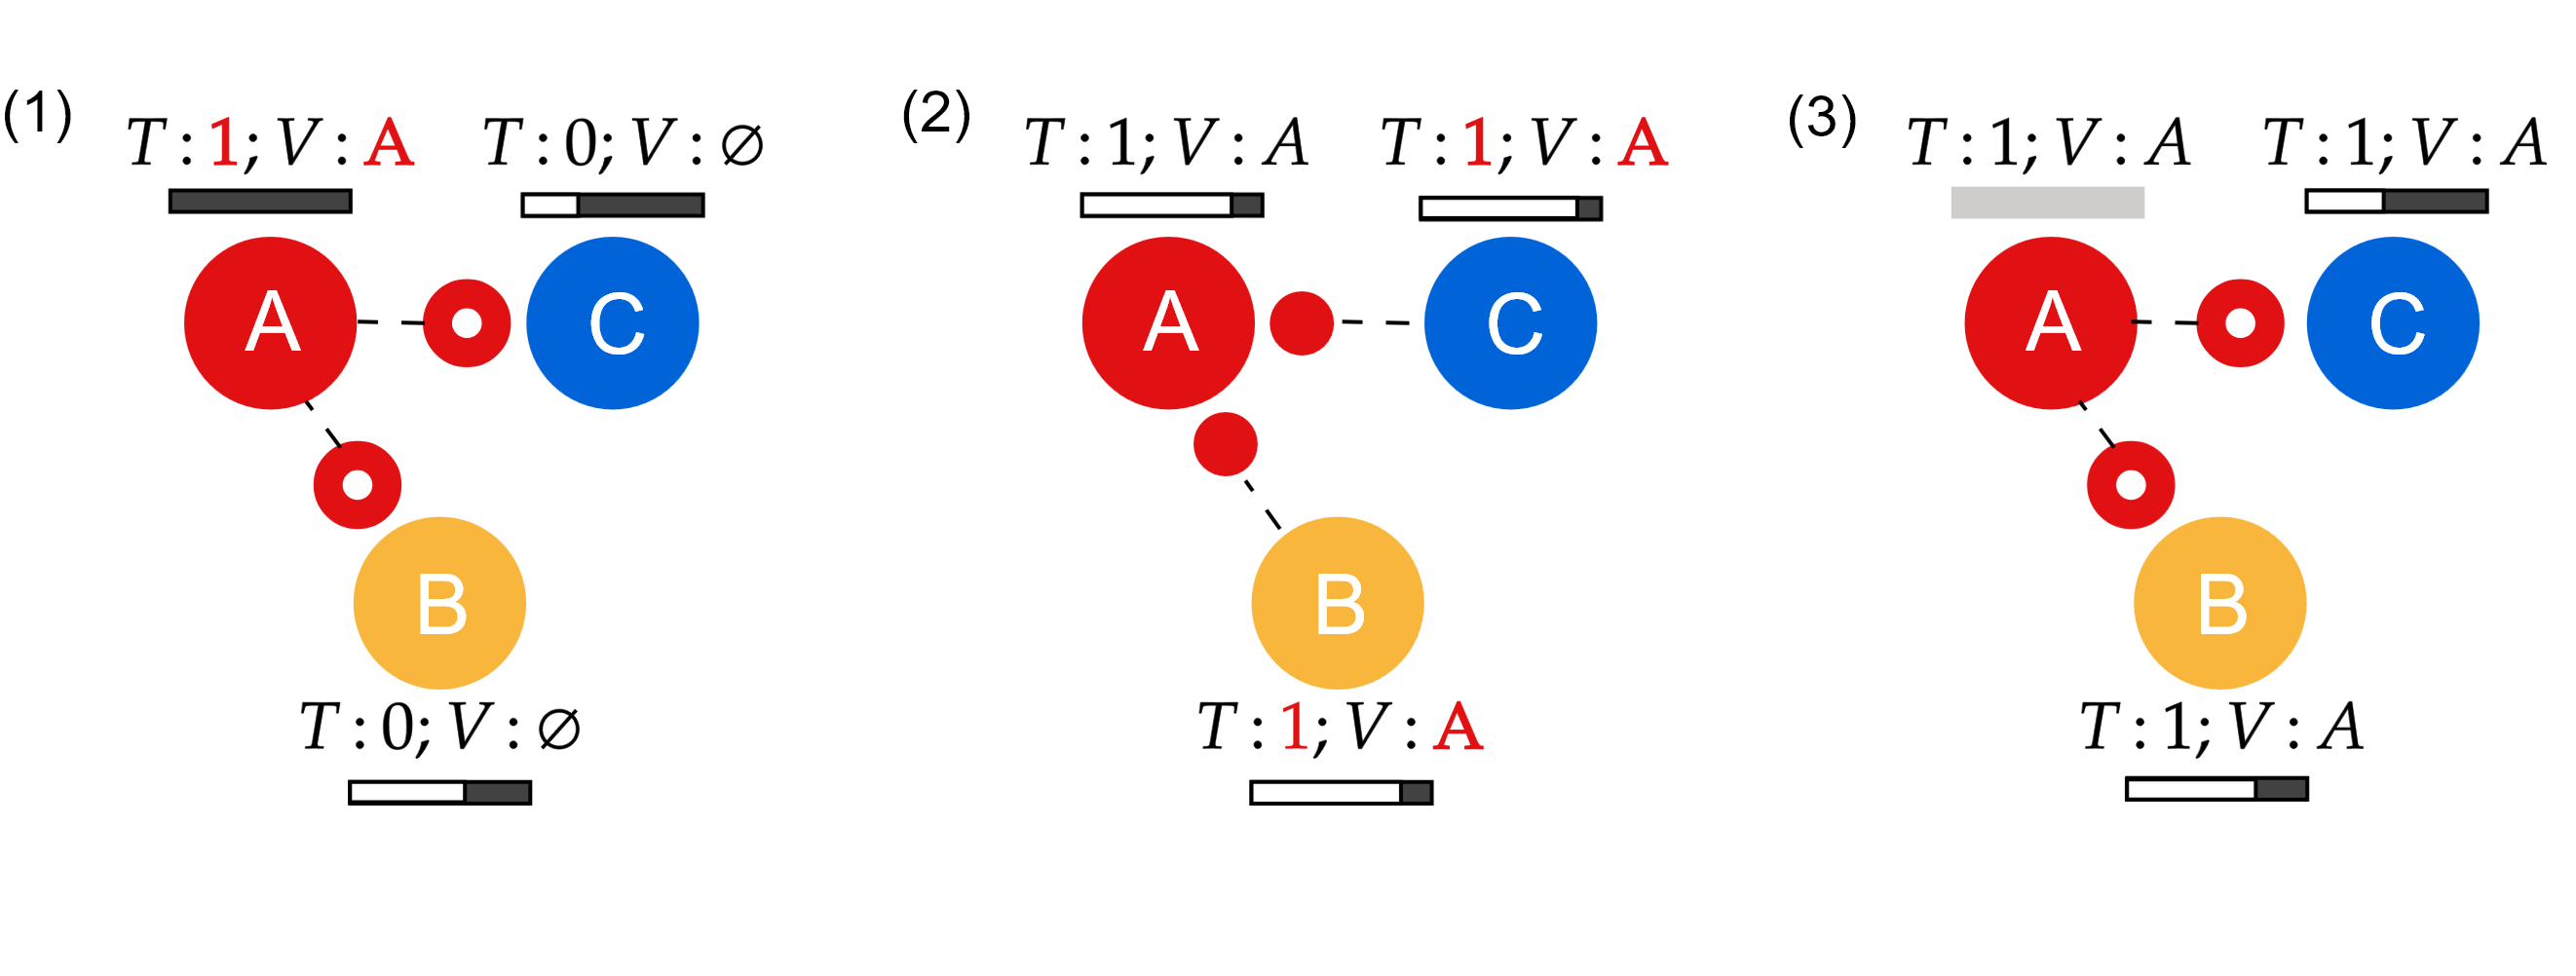
\includegraphics[width=\textwidth]{Sections/raft/election.png}
    \caption{First Election after boot where $A$, $B$, and $C$ nodes in a cluster of three have been initialized. 
    (1) $A$ times out first, becoming a Candidate and sending a RequestVote RPC to $B$ and $C$. (2) $B$ and $C$ vote for $A$.
    (3) $A$ receives the majority vote and becomes the Leader. Now $A$'s timer is no longer used.}
\end{figure}

\newpage

\noindent
Observe a cluster of four who is dealing with a split vote:
\begin{figure}[h]
    \centering
    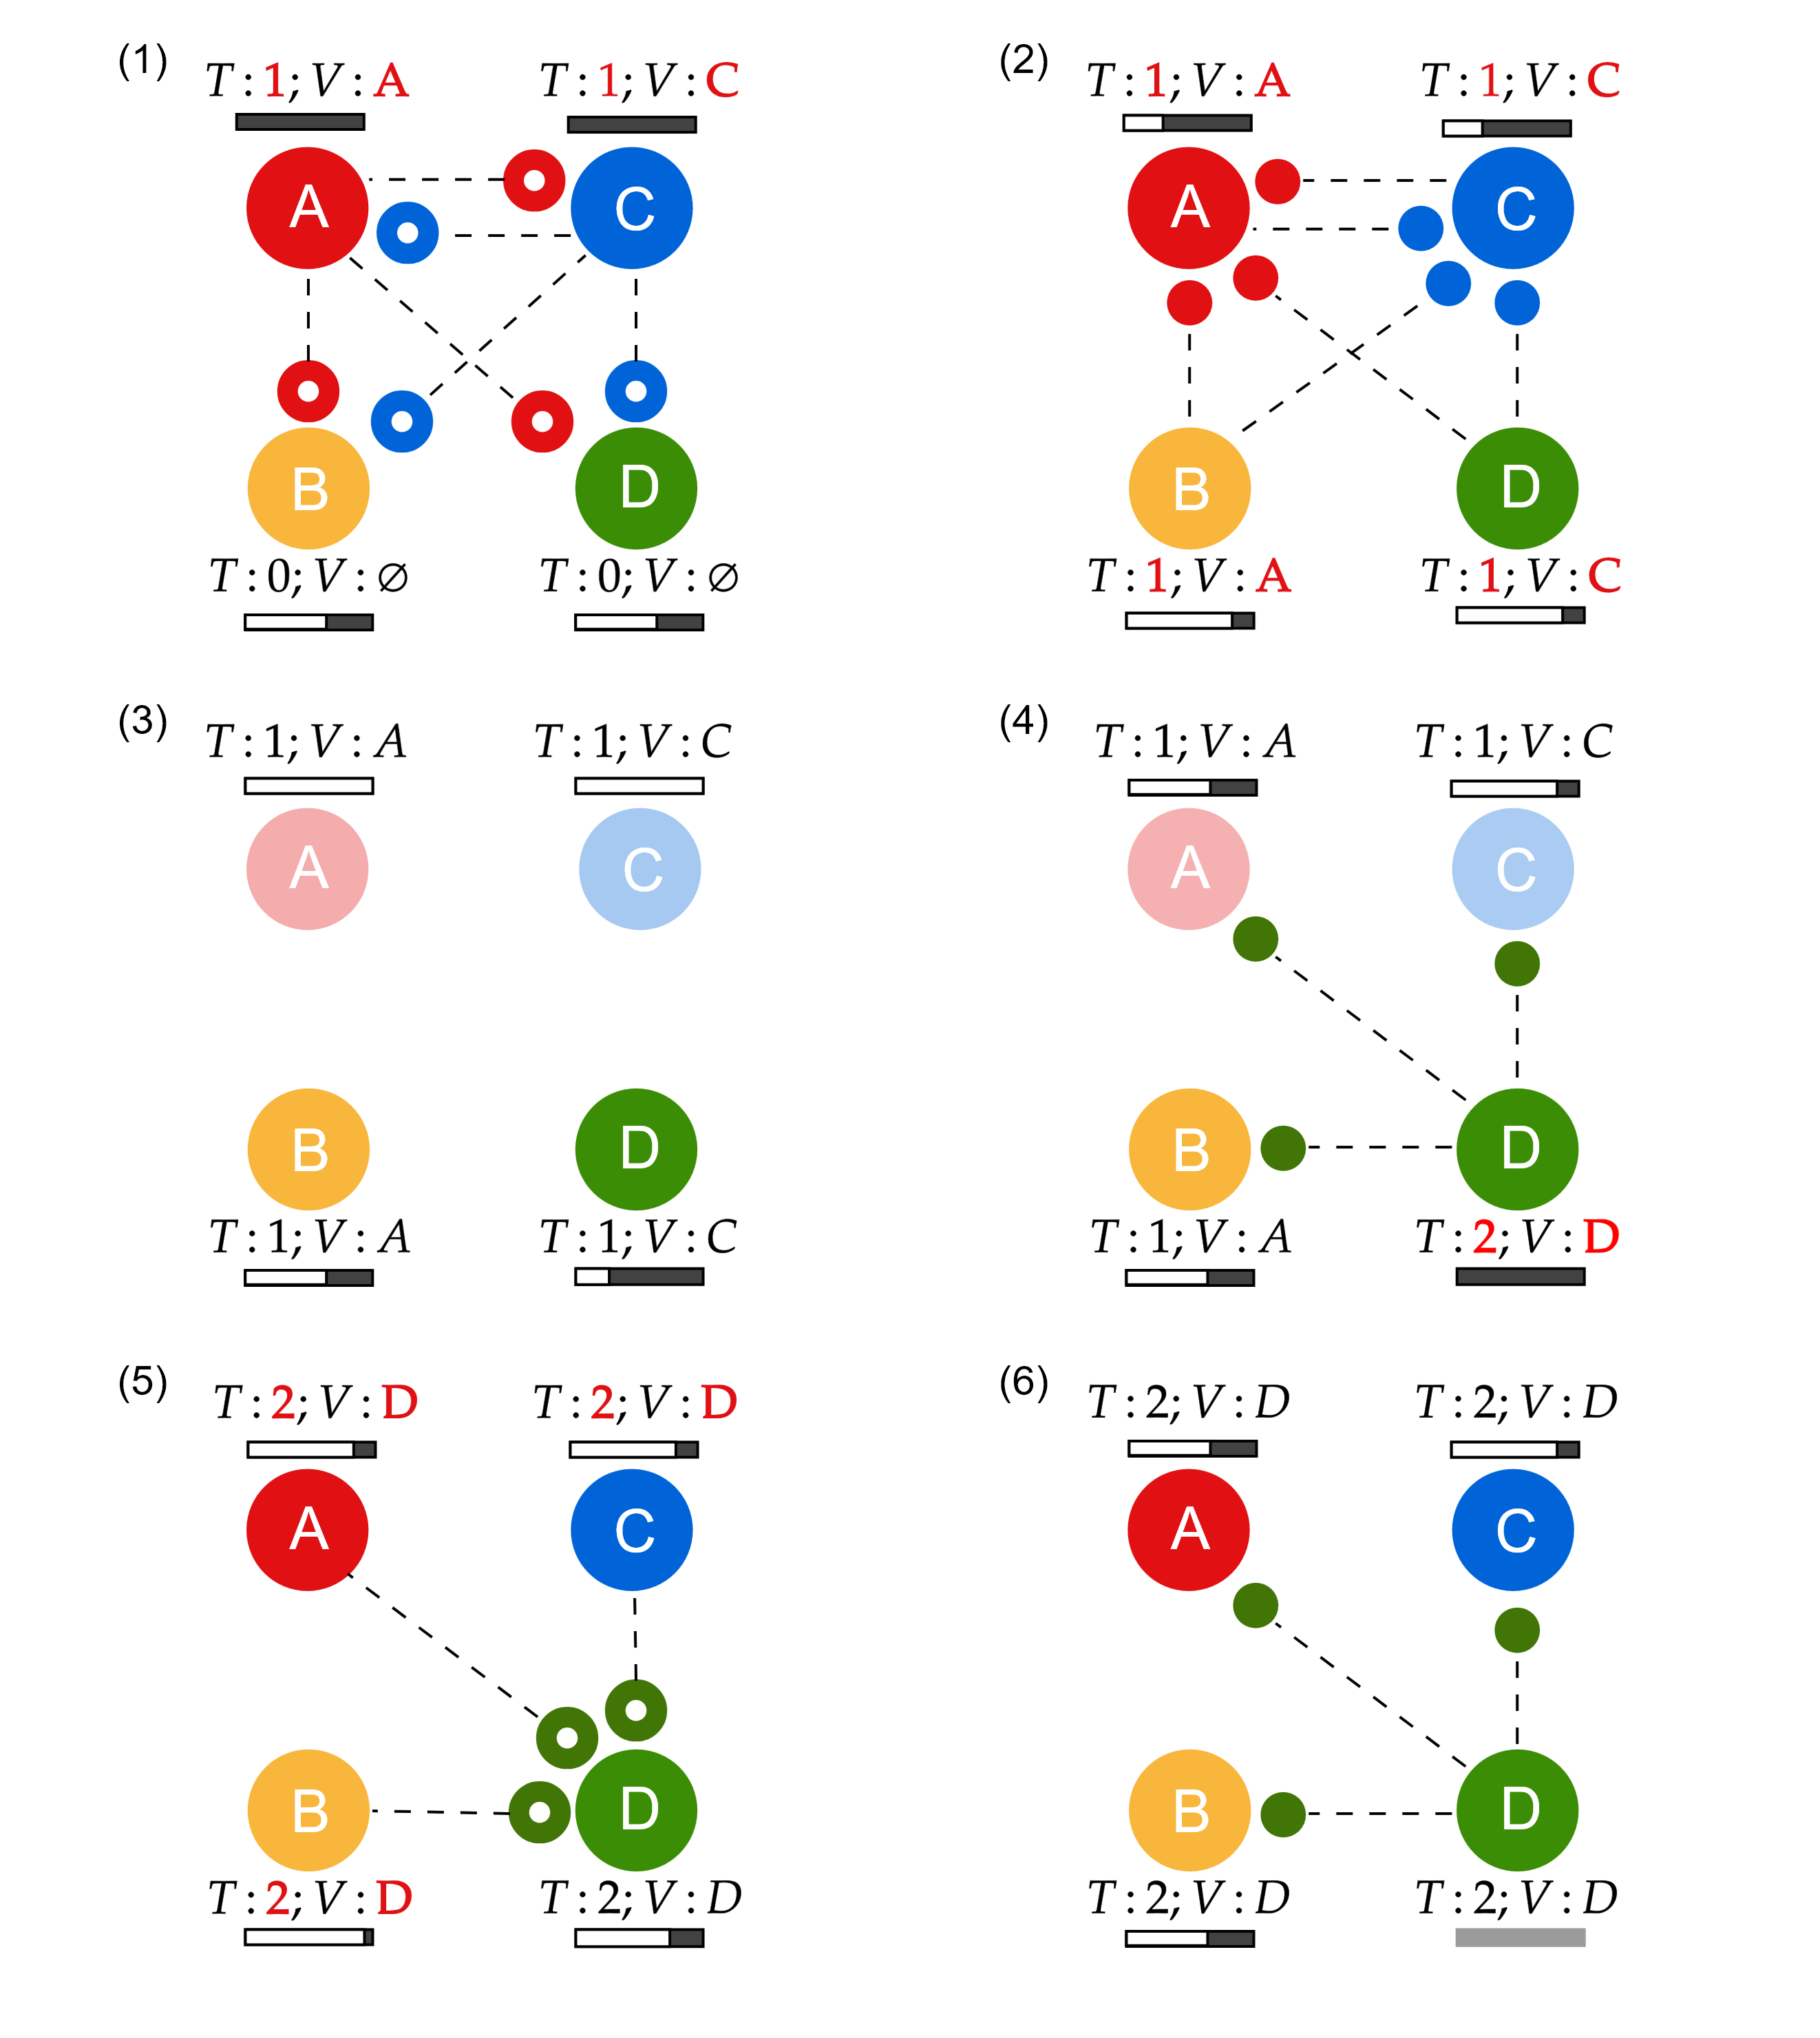
\includegraphics[width=.9\textwidth]{Sections/raft/split.png}
    \caption{(1) $A$ and $C$'s timers run out first, sending out a RequestVote RPC to all other servers. (2) $B$ votes for $A$, and $D$ votes for $C$. (3) $A$ and $C$ timeout as per split vote. 
    (4) $D$ times out starting a new term, casting their Request RPC. (5) All servers respond to the higher order term. (6) $D$ becomes the Leader (Their time no longer used).}
\end{figure}

\newpage
\begin{Def}[Log Replication]

    Given $\{\ \beta\ (\text{Server}): \gamma\ (\text{Follower})  |\ \varsigma\ (\text{Candidate}) |\ \ell\ (\text{Leader})\ \}$, the Raft Log Replication Process involves the following:
    \begin{itemize}
        \item \textbf{Leader Log Replication:} Once a $\ell$ is elected, it services command requests from the client. The $\ell$ first appends the command to its \textbf{indexed log},
        then sends an \textbf{AppendEntries RPC} in parallel to all $\beta$. Once a majority of $\beta$ have replicated the log, the command is \textbf{committed}, and thus, safe to apply to their state machine. 
        \item \textbf{Order of Execution:} The $\ell$ maintains a \snippet{nextIndex[]},
        indicating the next expected log entry for all $\beta$. The $\ell$ sends missing log entries to lagging $\beta$; otherwise, it sends empty \textbf{AppendEntries RPCs} as heartbeats.
        \item \textbf{Leader Redirection:} All $\beta$ that receive client requests, redirect the client to the $\ell$. 
    \end{itemize}
\end{Def}

\begin{theo}[Log Matching Property]

    \label{theo:log}
    If two entries in different logs have the same index and term, then:
    \begin{itemize}
        \item They store the same command.
        \item All proceeding entries are the same.
    \end{itemize}
\end{theo}

\begin{Def}[Log Correction]

    Given $\{\ \beta\ (\text{Server}): \gamma\ (\text{Follower})  |\ \varsigma\ (\text{Candidate}) |\ \ell\ (\text{Leader})\ \}$,\\

    \noindent
    If $\ell$ fails, the new $\ell$ may be missing log entries. Let $i$ denote the last index of $\ell$'s log entry, and $j$ the last index of other $\beta$s' logs.
    If after an \textbf{AppendEntries RPC}, $\beta$'s $j\neq i$, then $\ell$ decrements $\beta$'s \textbf{nextIndex} to $(j-1)$ \textbf{per call}, until $j=i$.
    Once majority coherence is met, the log is committed.\\

    \noindent
    This holds as we assume the preceding Theorem (\ref{theo:log}) is true. This is to say, the leader has a---\textbf{Append Only Property}---that it does not modify its own entries, but \textbf{only} appends new ones.
\end{Def}

\vspace{-.5em}
\begin{Note} 

    \textbf{Note:} A slight optimization for log correction, is for $\gamma$ to tell $\ell$ the conflicting term and its first index.
    With that, $\ell$ can skip the log entries of such term. Though this isn't necessary as in real world applications, these conflicts are 
    infrequent.
\end{Note}

\noindent


\newpage 

\subsection{Safety: Restricting Leader Election}
\noindent
Since previously discussed, a new leader may be missing log entries, from which they tell other servers to discard mismatches. 
This can become problematic when the previous leader and other servers have committed several entries.\\

\noindent
To fix this, we introduce constraints on leader election:

\begin{Def}[Leader Completeness]

    All proceeding leaders must have all committed entries of the previous leader.
\end{Def}

\begin{Def}[Leader Election Restriction]

    Given $\{\ \beta\ (\text{Server}): \gamma\ (\text{Follower})  |\ \varsigma\ (\text{Candidate}) |\ \ell\ (\text{Leader})\ \}$,\\
    New $\ell$ must demonstrate \textbf{Leader Completeness}. To ensure this, $\beta$ upon receiving a \textbf{RequestVote RPC} from $\varsigma$ checks:
    \begin{itemize}
        \item If $\varsigma$'s last log is from a lower term, the vote is \textbf{rejected}.
        \item If $\varsigma$'s last log is from the same term, but shorter, the vote is \textbf{rejected}.
        \item If $\varsigma$'s last log is from a higher term, then the vote is \textbf{accepted}.
        \item If $\varsigma$'s log is \textbf{at least} as up-to-date as the voter, the vote is \textbf{accepted}.
    \end{itemize}
\end{Def}

\begin{theo}[Present Term Commitment]

    Leaders cannot assume previous term entries are committed, as they may not have been fully replicated.
    Hence they only commit entries from their term, and by the \textbf{Log Matching Property} (\ref{theo:log}), previous entries are also committed.
\end{theo}

\begin{theo}[Ensuring a Leader Through Timing]

    To ensure that there is always a leader in the face of probabilistic timing, these 
    magnitude requirements should be satisfied:
    $$
    broadcastTime \ll electionTimeout \ll MTBF
    $$
    \noindent
    $broadcastTime$ measures the average time of heartbeat reciprocation (e.g., .5ms-20ms).
    Then $electionTimeout$, the randomly assigned timeout times for each server (e.g, 10ms-500ms), and $MTBF$, the
    average time between failures of a server (e.g., several months or more).
\end{theo}

\newpage 

\subsection{AppendEntries, State, and RequestVote RPC Schema}

\noindent
The next two pages are a summary of the Raft RPCs \textbf{AppendEntries}, \textbf{RequestVote}, and \textbf{state} for implementation:\\

\vspace{2em}

\noindent
\resizebox{\textwidth}{!}{%
    
    \renewcommand{\arraystretch}{1.6} % Increased padding
    \begin{tabular}{|l|p{9cm}|}
        \hline
        \rowcolor{Black} \multicolumn{2}{|c|}{\textcolor{white}{\textbf{AppendEntries RPC}}} \\
        \hline
        \rowcolor{OliveGreen!10}\multicolumn{2}{|l|}{\textbf{Invoked by leader to replicate log entries; also used as heartbeat.}} \\
        \hline
        \rowcolor{OliveGreen!10} \textbf{Arguments} & \hspace{12em}\textbf{Description} \\
        \hline
        \textbf{term} & Leader's term. \\
        \hline
        \textbf{leaderId} & Allows follower to redirect clients. \\
        \hline
        \textbf{prevLogIndex} & Index of log entry immediately preceding new ones. \\
        \hline
        \textbf{prevLogTerm} & Term of \textbf{prevLogIndex}, entry. \\
        \hline
        \textbf{entries[]} & Log entries to store (empty for heartbeat; may send more than one for efficiency). \\
        \hline
        \textbf{leaderCommit} & Leader's \textbf{commitIndex}. \\
        \hline
        \rowcolor{OliveGreen!10} \textbf{Results} &  \\
        \hline
        \textbf{term} & Current term, for leader to update itself. \\
        \hline
        \textbf{success} & \textbf{true} if follower contained entry matching \textbf{prevLogIndex} and \textbf{prevLogTerm}. \\
        \hline
        \rowcolor{OliveGreen!10} \textbf{Receiver Implementation} & \\
        \hline
        \multicolumn{2}{|p{10cm}|}{%
            \parbox{11cm}{%
                \begin{enumerate}
                    \item Reply \textbf{false} if \textbf{term} $<$ \textbf{currentTerm}.
                    \item Reply \textbf{false} if log doesn't contain an entry at \textbf{prevLogIndex} whose term matches \textbf{prevLogTerm}.
                    \item If an existing entry conflicts with a new one (same index but different terms), delete the existing entry and all that follow it.
                    \item Append any new entries not already in the log.
                    \item If \textbf{leaderCommit} $>$ \textbf{commitIndex}, set \textbf{commitIndex} $=\min(\text{\textbf{leaderCommit}}, \text{index of last new entry})$.
                \end{enumerate}
            }
        } \\
        \hline
    \end{tabular}
}

\newpage
    \resizebox{\textwidth}{!}{%
    \renewcommand{\arraystretch}{1.6} % Increased padding
    \begin{tabular}{|l|p{9cm}|}
        \hline
        \rowcolor{Black}\multicolumn{2}{|c|}{\textcolor{white}{\textbf{STATE}}}\\
        \hline
        \rowcolor{OliveGreen!10}\multicolumn{2}{|c|}{\textbf{Persistent state on all servers (stored on stable storage before responding to RPCs)}} \\
        \hline
        \textbf{currentTerm} & Latest term server has seen (initialized to 0 on first boot, increases monotonically). \\
        \hline
        \textbf{votedFor} & Candidate ID that received vote in current term (or null if none). \\
        \hline
        \textbf{log[]} & Log entries; each entry contains a command for the state machine and the term when it was received by the leader (first index is 1). \\
        \hline
        \rowcolor{OliveGreen!10}\multicolumn{2}{|c|}{\textbf{Volatile state on all servers}} \\
        \hline
        \textbf{commitIndex} & Index of the highest log entry known to be committed (initialized to 0, increases monotonically). \\
        \hline
        \textbf{lastApplied} & Index of highest log entry applied to the state machine (initialized to 0, increases monotonically). \\
        \hline
        \rowcolor{OliveGreen!10}\multicolumn{2}{|c|}{\textbf{Volatile state on leaders (Reinitialized after election)}} \\
        \hline
        \textbf{nextIndex[]} & For each server, index of the next log entry to send to that server (initialized to leader last log index + 1). \\
        \hline
        \textbf{matchIndex[]} & For each server, index of highest log entry known to be replicated on server (initialized to 0, increases monotonically). \\
        \hline
        \rowcolor{Black} \multicolumn{2}{|c|}{\textcolor{white}{\textbf{RequestVote RPC}}} \\
        \hline
        \rowcolor{OliveGreen!10}\multicolumn{2}{|l|}{\textbf{Invoked by candidates to gather votes.}} \\
        \hline
        \textbf{term} & Candidate's term. \\
        \hline
        \textbf{candidateId} & Candidate requesting vote. \\
        \hline
        \textbf{lastLogIndex} & Index of candidate's last log entry. \\
        \hline
        \textbf{lastLogTerm} & Term of candidate's last log entry. \\
        \hline
        \rowcolor{OliveGreen!10} \textbf{Results} &  \\
        \hline
        \textbf{term} & Current term, for candidate to update itself. \\
        \hline
        \textbf{voteGranted} & \textbf{true} means candidate received vote. \\
        \hline
        \rowcolor{OliveGreen!10} \textbf{Receiver Implementation} & \\
        \hline
        \multicolumn{2}{|p{9cm}|}{%
            \parbox{11cm}{%
                \begin{enumerate}
                    \item Reply \textbf{false} if \textbf{term < currentTerm}.
                    \item If \textbf{votedFor} is \textbf{null} or \textbf{candidateId}, and candidate's log is at least as up-to-date as receiver's log, grant vote.
                \end{enumerate}
            }
        } \\
        \hline
    
    \end{tabular}
}

\newpage
\clearpage

\begin{figure}[ht!]
    \centering
    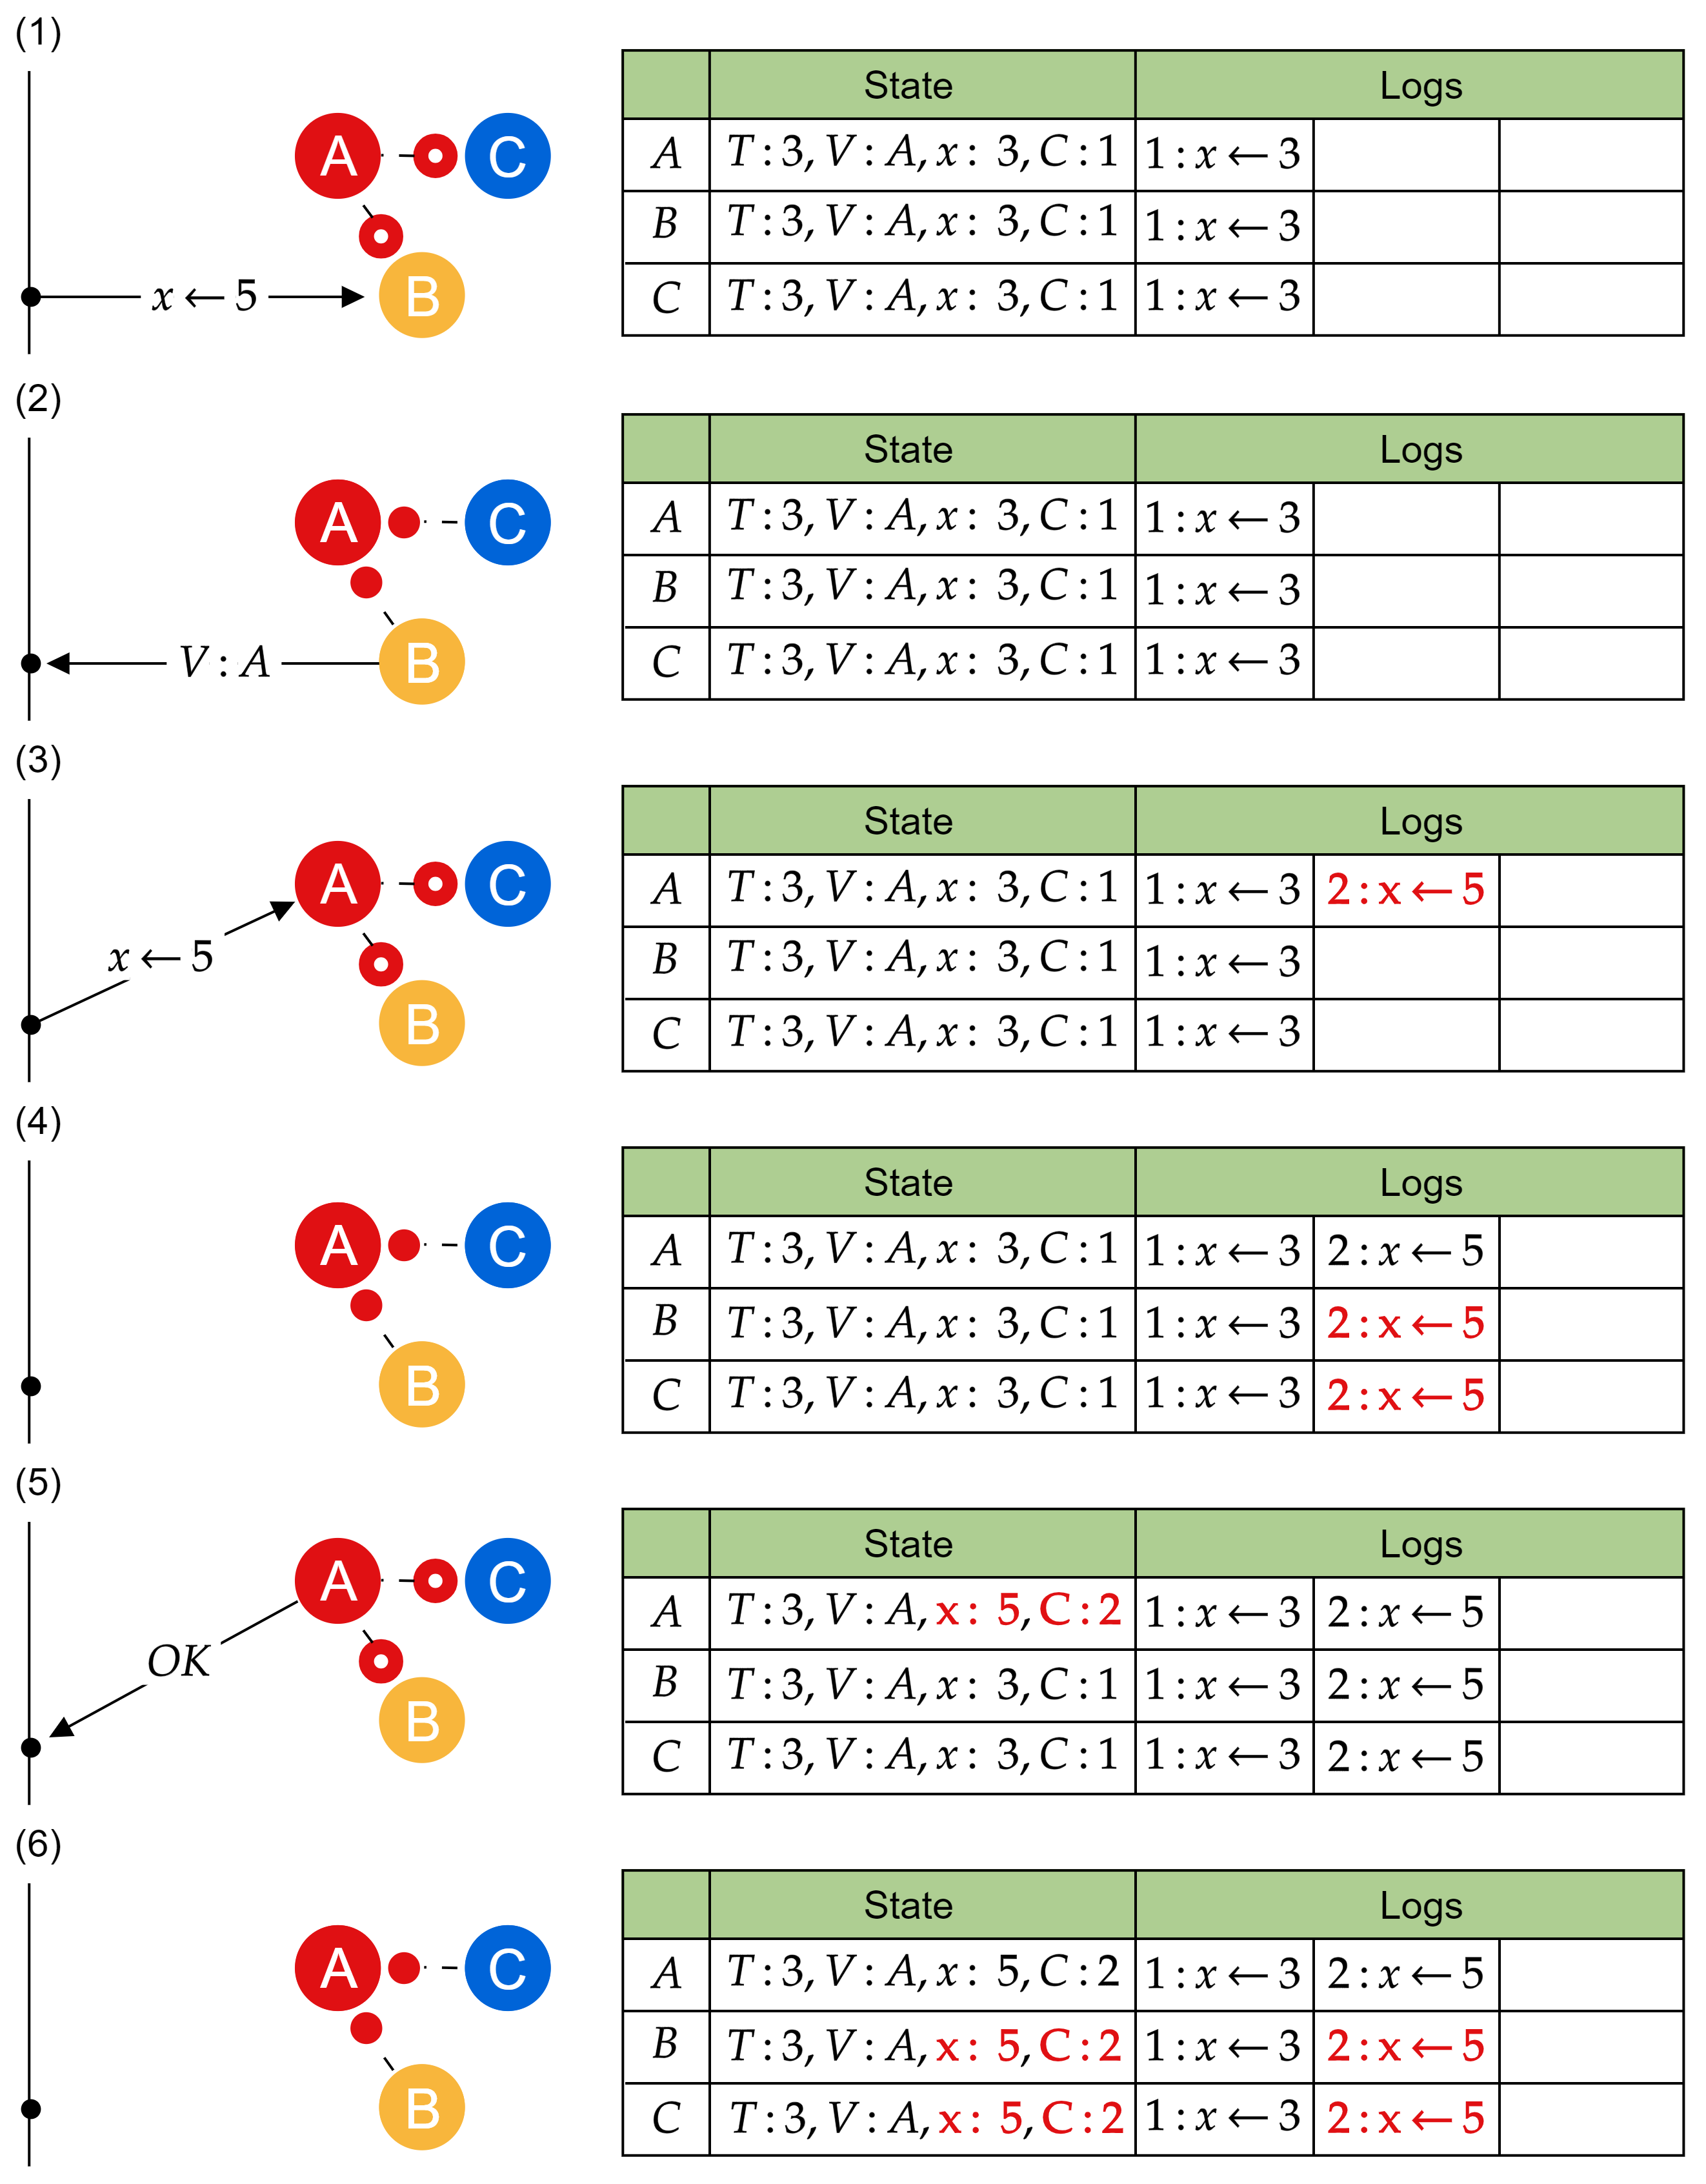
\includegraphics[width=.869\textwidth]{Sections/raft/logs.png}
    \caption{Simplified Raft server log replication where $T$ is the current term, $V$ is the voted for candidate, and $C$ is the commit index. (1-3) The client's request is redirected from $B$ to $A$. 
    Then $A$ propagates the command $x\leftarrow 5$ as log index 2. (4) both $B$ and $C$ replicate the log and send back a heartbeat. (5) $A$ commits log 2, applies it to state, and sends an acknowledgment back to the client.
    (6) $B$ and $C$ update the newly committed index and apply it to state.}
\end{figure}
\newpage

\begin{figure}[ht!]
    \centering
    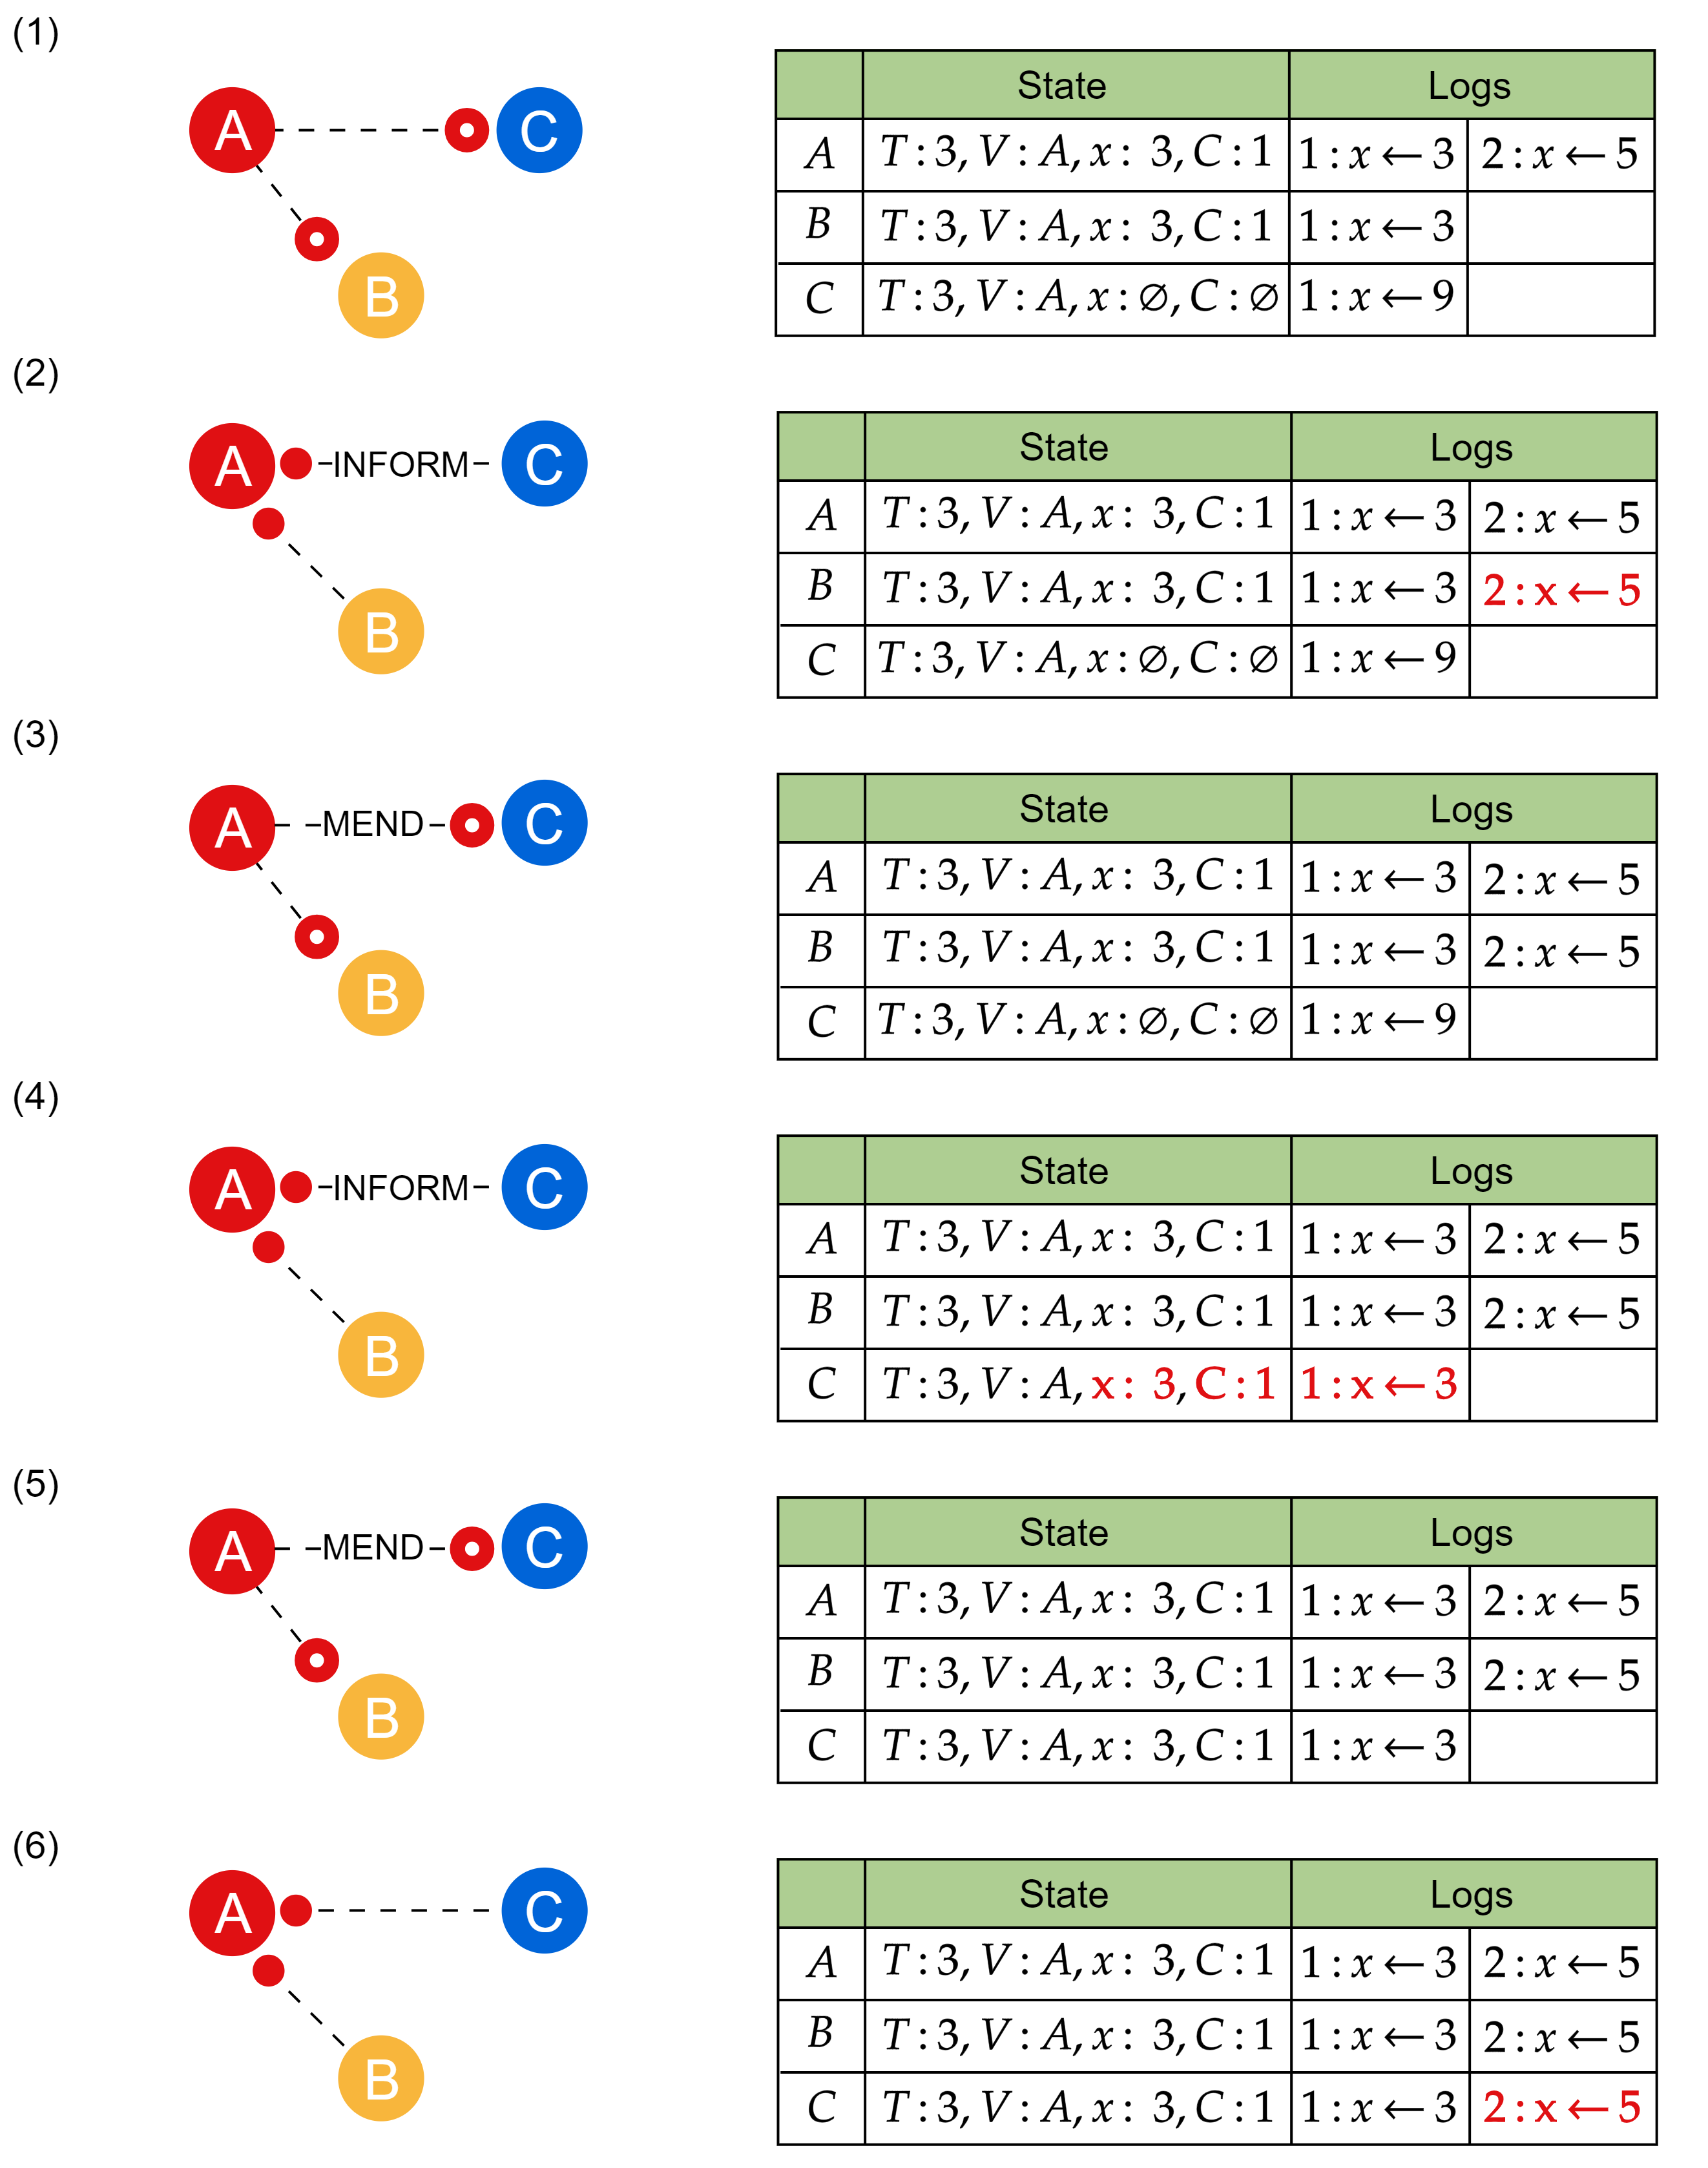
\includegraphics[width=.869\textwidth]{Sections/raft/logs_2.png}
    \caption{(1) Server $C$ has an incorrect log, whilst server $A$ sends out the command $x\leftarrow 5$. (2) Server $C$ receives the command, but rejects it and informs $A$ where they differ. (3) Server $A$ re-sends the log from which they differ. 
    (4) Server $C$ corrects such entry, and informs $A$ again. (5) Server $A$ retries once more. (6) Server $C$ receives the log and replicates it, and is thus up-to-date.}
\end{figure}

\newpage
\subsection{Cluster Reconfiguration (Adding, Removing, and Replacing Servers)}
\noindent
Cluster reconfiguration involves adding, removing, and replacing servers, or adjusting routines:

\begin{Def}[Stop and Restart \& Pause and Resume]

    \begin{itemize}
        \item \textbf{Stop and Restart:} Immediately halt operations, save state, reconfigure, and restart.
        \item \textbf{Pause and Resume:} Pause executing incoming requests and instead save them in a buffer, finish current processes,
        reconfigure, restart and resume. 
    \end{itemize}
\end{Def}

\noindent
Raft takes a two phase approach to reconfigure the cluster:
\begin{Def}[Raft Joint Consensus Reconfiguration (Part 1)]

    Joint consensus allows for a cluster to service requests while reconfiguring.
    It does this via a transition state, which is a combination of the old and new configurations (Joint consensus).\\

    \noindent
    \textbf{Reconfiguration:} Once a leader receives a configurations request to swap from $C_{old}$ to $C_{new}$, it appends $C_{old,new}$ to its logs, proceeding
    as follows:
    \begin{itemize}
        \item \textbf{Phase 1:}
        \begin{enumerate}
            \item Propagate $C_{old,new}$ to all servers.
            \item Servers receiving new configurations (e.g., $C_{old,new}$), acknowledge it (\textbf{regardless} if it's committed or not).
            \item A leader crashing leads to reelections under $C_{old}$ or $C_{old,new}$.
            \item Once $C_{old,new}$ is committed, the leader appends $C_{new}$ to its log and replicates it.
        \end{enumerate}
        \item \textbf{Phase 2:} 
        \begin{enumerate}
            \item $C_{new}$ is committed and live, any server not under $C_{new}$ can be shut down.
            \item The leader who committed $C_{new}$ becomes a follower to account for \textbf{Deletion}.
        \end{enumerate}
        
        
    \end{itemize}

    \noindent
    \textbf{Deletion:} To remove servers, they are excluded in the $C_{new}$ configuration; \textbf{With the only exception} that leaders who do not exist in $C_{new}$
    \underline{may continue to manage the cluster} until $C_{new}$ is committed.\\
    
    \noindent
    \textbf{Addition:} New Servers enter with \textbf{empty logs} and are added in the following manner:
    \begin{enumerate}
        \item The leader upon receiving the $C_{new}$ request is notified of new server existence.
        \item New servers \textbf{cannot vote}, but only receive logs (as to avoid splitting the cluster).
        \item Once new servers are synchronized in logs, $C_{old,new}$ may be committed.
        \item $C_{old,new}$ clusters require the majority vote from \textbf{both old and new servers}.
    \end{enumerate}
\end{Def}
\newpage

\noindent
Though we must address the situation where servers outside of $C_{new}$ try to 
cast votes:
\begin{Def}[Raft Joint Consensus Reconfiguration (Part 2)]

    Since Raft processes requests asynchronously, during the transition to the new configuration 
    from $C_{old,new}$ to $C_{new}$, the following could happen:
    \begin{itemize}
        \item A server not yet notified of the new configuration may not know it has been removed from it.
        Hence, it may not receive heartbeats and attempt to start a new election.
        \item A server with some other configuration comes online and begins to send out RPCs to the cluster.
    \end{itemize}

    \noindent
    In any such case of unwanted votes, Raft enacts the following protocol to ensure safety:
    \begin{itemize}
        \item \textbf{Leader Liveliness:} If servers within $C_{new}$ believe they have a leader, they ignore votes \underline{(regardless of higher order terms).}
        \item \textbf{Majority Rule:} Even if an election occurs, $C_{new}$ members will vote amongst themselves, for which servers outside of $C_{new}$ will never win.
    \end{itemize}

    \noindent
    Ideally, we would like to immediately terminate servers that are removed, but this may not always be possible or practical.
\end{Def}

\vspace{-1em}
\noindent
\subsection{Log Compaction \& Snapshotting}

\noindent
In finite systems, logs cannot expand without bound. So as to clean log entries without losing state consensus, snapshotting is employed.
\begin{Def}[Raft - Log Compaction \& Snapshots]

    Raft compacts logs via state snapshots (\ref{def:snapshot}). Servers independently take snapshots, and \textbf{are} \underline{\textbf{not} initiated by the leader.}
    Snapshots employ the following protocol:
    \begin{enumerate}
        \item Trigger snapshots when logs reach a fixed size in \textbf{bytes} or time (e.g., see below tip).
        \item The snapshot replaces \textbf{committed} log entries and retains entries yet to be committed.
        \item The snapshot includes last committed log index, term of last index, and machine state\\
        (e.g., key-value pairs).
    \end{enumerate}
\end{Def}
\begin{Tip} \textbf{Simple Snapshot Initiate Protocol} - One possible 
    solution suggested by the Raft paper is to initiate the snapshot when the log reaches a certain size in bytes.
    Ideally a size significantly larger than the size of the expected snapshot. Since snapshots have a \textbf{fixed cost}
    in setup, it reduces the overall cost overtime if snapshots occur at fewer intervals.
\end{Tip}

\newpage 

\noindent
\begin{Proof}[Raft - Log Compaction \& Snapshots]

    Leader initiated snapshots may overcomplicate its RPC and or make costly use of
    bandwidth. Since the leader has already vetted committed 
    log entries, it is safe to assume that the resulting independent snapshots consisting of committed logs---are also safe. 
\end{Proof}

\noindent
Though it's not ideal to send an snapshots over the network, in some cases we might have to.
\begin{Def}[Raft Resynchronization (InstallSnapshot RPC)]

    There are two cases where a snapshot may be sent:
    \begin{enumerate}
        \item \textbf{Missing Entry}: If the leader has already compacted a log entry it needs to send to a server, it sends the snapshot instead.
        \item \textbf{Server Recovery}: A server coming online may be severely behind, and thus, simply sending AppendEntries RPCs may take too long.
    \end{enumerate}

    \noindent
    In such cases the leader will send a \textbf{InstallSnapshot RPC}.
    Such RPC includes the last log index. The receiver discards all its logs before the last 
    log index, and retains the rest.
\end{Def}

\noindent
Copying the entire dataset is costly, as to avoid this, Raft recommends a lazy snapshotting approach:

\begin{Def}[Copy-on-Write (CoW)]

    \noindent
    Servers mark existing data as shared between a snapshot and live state.
    Only when a write (modification) touches shared data, does the server copy to preserve the snapshot.
\end{Def}

\begin{Def}[Raft - Handling Stale Logs in Client Interactions]

    \noindent
    Raft ensures clients receive up-to-date logs from leaders via the following methods:

    \begin{itemize}
        \item \textbf{Command IDs:} Each command is assigned unique serial numbers. Each server maintains the last processed command ID and associated response for 
        each client.
        \item \textbf{Syncing Leader Logs:} To avoid stale leader logs, two precautionary are taken: 
        \begin{enumerate}
            \item At the beginning of each term, the leader replicates a dummy \textit{no-op} command log and waits for it to be committed.
            \item The leader sends responses only after exchanging heartbeats with the majority.
        \end{enumerate}
    \end{itemize}
\end{Def}
    
\newpage

\subsection{InstallSnapshot RPC Schema}

\noindent
Below is a summary of the Raft RPC \textbf{InstallSnapshot} for implementation:\\

\vspace{2em}

\noindent
\resizebox{\textwidth}{!}{%
    \renewcommand{\arraystretch}{1.6} % Increased padding
    \begin{tabular}{|l|p{13.3cm}|}
        \hline
        \rowcolor{Black} \multicolumn{2}{|c|}{\textcolor{white}{\textbf{InstallSnapshot RPC}}} \\
        \hline
        \rowcolor{OliveGreen!10}\multicolumn{2}{|l|}{\textbf{Invoked by leader to send chunks of a snapshot to a follower. Leaders always send chunks in order.}} \\
        \hline
        \rowcolor{OliveGreen!10} \textbf{Arguments} & \hspace{12em}\textbf{Description} \\
        \hline
        \textbf{term} & Leader's term. \\
        \hline
        \textbf{leaderId} & Allows follower to redirect clients. \\
        \hline
        \textbf{lastIncludedIndex} & The snapshot replaces all entries up through and including this index. \\
        \hline
        \textbf{lastIncludedTerm} & Term of \textbf{lastIncludedIndex}. \\
        \hline
        \textbf{offset} & Byte offset where chunk is positioned in the snapshot file. \\
        \hline
        \textbf{data[]} & Raw bytes of the snapshot chunk, starting at \textbf{offset}. \\
        \hline
        \textbf{done} & \textbf{True} if this is the last chunk. \\
        \hline
        \rowcolor{OliveGreen!10}\multicolumn{2}{|l|}{\textbf{Response to Sender}} \\
        \hline
        \textbf{term} & Current term, for leader to update itself. \\
        \hline
        \rowcolor{OliveGreen!10}\multicolumn{2}{|l|}{\textbf{Reciever Implementation}} \\
        \hline
        \multicolumn{2}{|p{10cm}|}{%
            \parbox{11cm}{%
                \begin{enumerate}
                    \item Reply immediately if \textbf{term} $<$ \textbf{currentTerm}.
                    \item Create new snapshot file if first chunk (\textbf{offset} = 0).
                    \item Write data into snapshot file at given \textbf{offset}.
                    \item Reply and wait for more data chunks if \textbf{done} is false.
                    \item Save snapshot file, discard any existing or partial snapshot with a smaller index.
                    \item If existing log entry has the same index and term as snapshot's last included entry, retain log entries following it and reply.
                    \item Discard the entire log.
                    \item Reset state machine using snapshot contents (and load snapshot's cluster configuration).
                \end{enumerate}
            }
        } \\
        \hline
    \end{tabular}
}

\newpage

\noindent
Consider the below figure which illustrates a snapshot taken from a server $A$:
\begin{figure}[ht!]
    \centering
    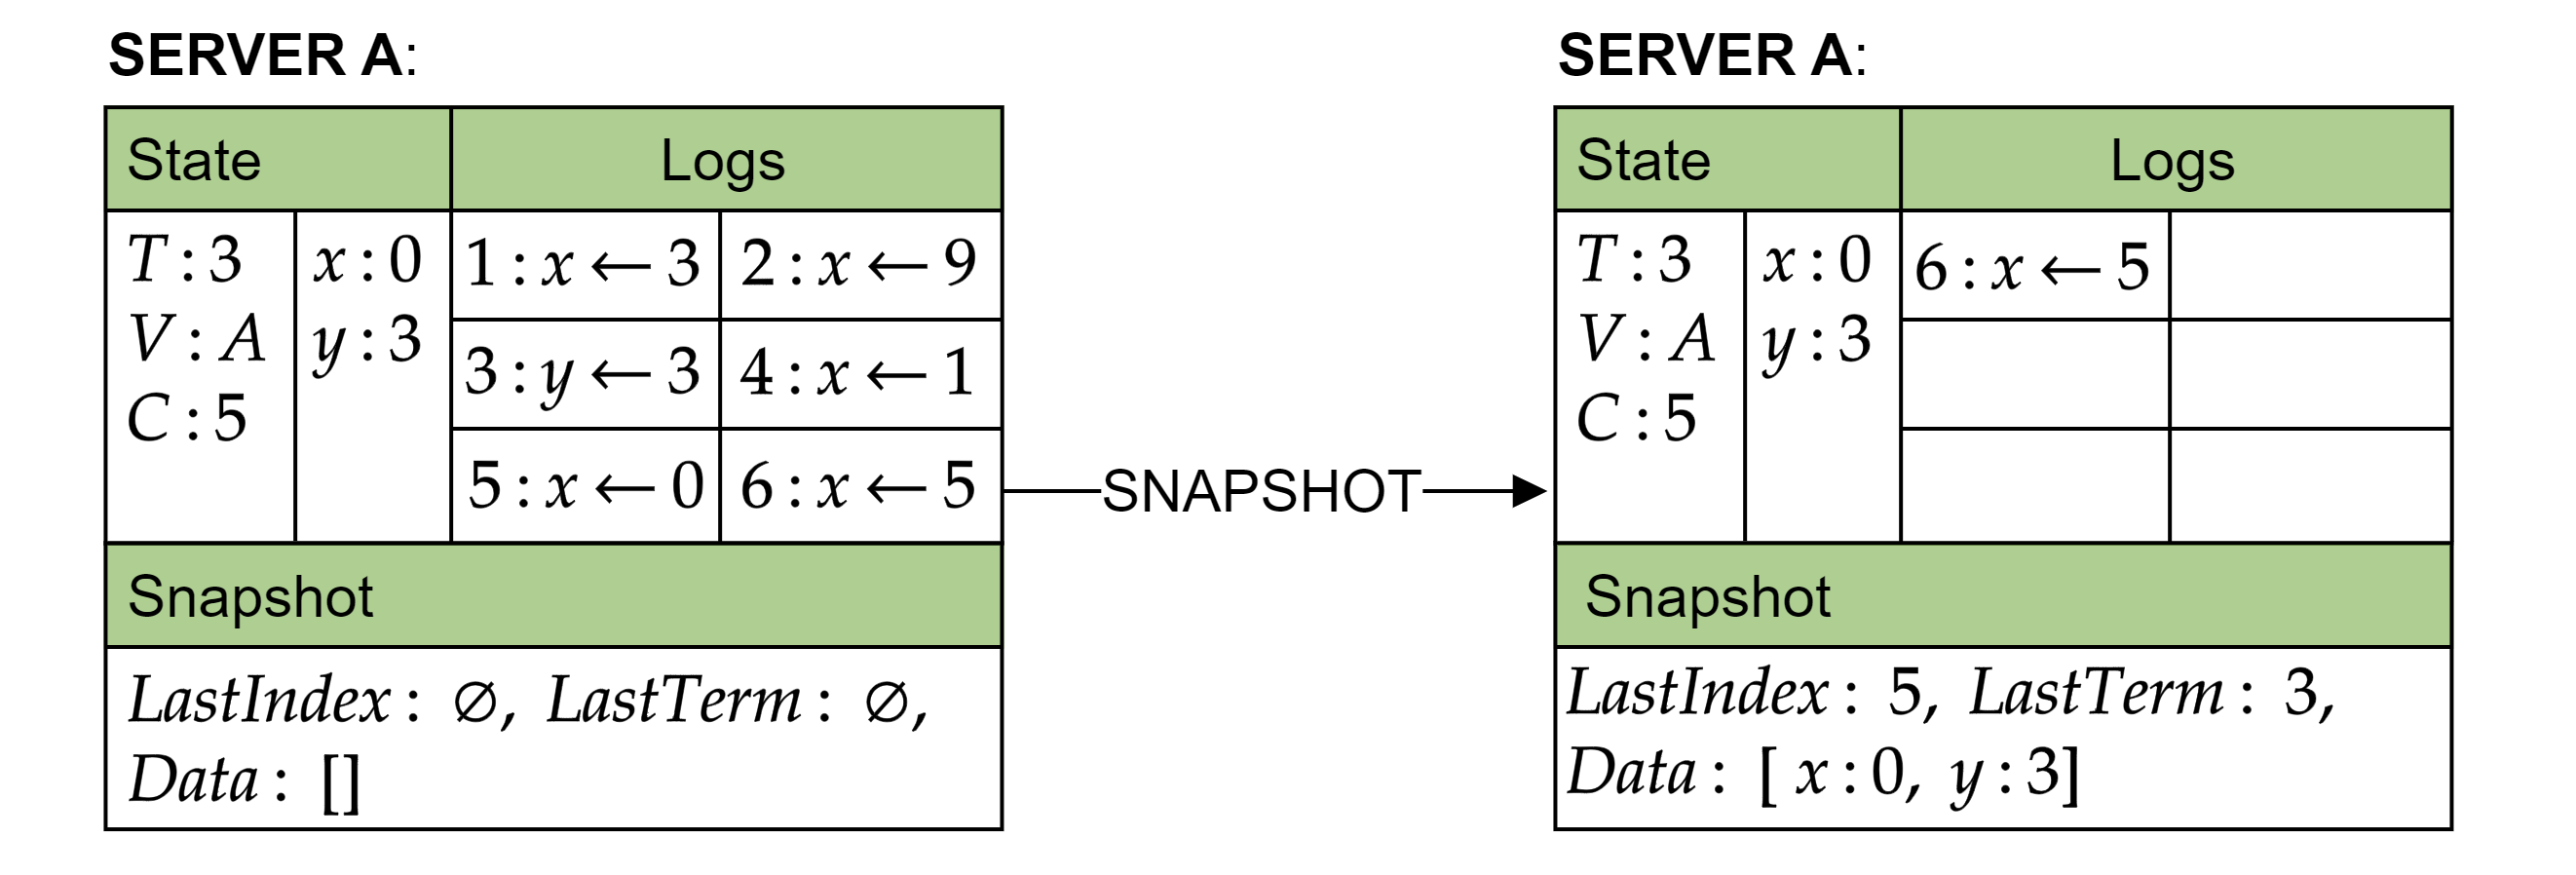
\includegraphics[width=\textwidth]{Sections/raft/snap.png}

    \vspace{1em}
    \caption{Server $A$ begins with the initial state where, $T$ is the current term, $V$ is the voted for candidate, and $C$ is the commit index. There is a separate partition for the snapshot where,
    $LastIndex$ is the last committed log entry's index, and $LastTerm$, the 
    term from which $LastIndex$ resided. The arrow points towards after the snapshot, from which we see 6, the remaining log entry that wasn't committed.}
\end{figure}


\subsection{Raft Algorithm Paper}
Below is the original source with additional proofs and explanations \cite{184040}:
\begin{itemize}
    \item \href{https://www.usenix.org/system/files/conference/atc14/atc14-paper-ongaro.pdf}{https://www.usenix.org/system/files/conference/atc14/atc14-paper-ongaro.pdf}
    \item \textbf{Extended Version:} \href{https://raft.github.io/raft.pdf}{https://raft.github.io/raft.pdf}
\end{itemize}

\noindent
And these two websites which offer interactive visualizations of the Raft Algorithm:
\begin{itemize}
    \item \href{http://thesecretlivesofdata.com/raft/}{http://thesecretlivesofdata.com/raft/}
    \item \href{https://raft.github.io/}{https://raft.github.io/}
\end{itemize}

